%Supplementary Information for the 2015 submission to Geophysical Research Letters with Jesse Day, Jake Edman, John Chiang, Inez Fung and Weihan Liu



%%%%%%%%%%%%%%%%%%%%%%%%%%%%%%%%%%%%%%%%%%%%%%%%%%%%%%%%%%%%%%%%%%%%%%%%%%%%
% AGUtmpl.tex: this template file is for s formatted with LaTeX2e,
% Modified November 2013
%
% This template includes commands and instructions
% given in the order necessary to produce a final output that will
% satisfy AGU requirements.
%
% PLEASE DO NOT USE YOUR OWN MACROS
% DO NOT USE \newcommand, \renewcommand, or \def.
%
% FOR FIGURES, DO NOT USE \psfrag
%
%%%%%%%%%%%%%%%%%%%%%%%%%%%%%%%%%%%%%%%%%%%%%%%%%%%%%%%%%%%%%%%%%%%%%%%%%%%%
%
% All questions should be e-mailed to latex@agu.org.
%
%%%%%%%%%%%%%%%%%%%%%%%%%%%%%%%%%%%%%%%%%%%%%%%%%%%%%%%%%%%%%%%%%%%%%%%%%%%%
%
% Step 1: Set the \documentclass
%
% There are two options for article format: two column (default)
% and draft.
%
% PLEASE USE THE DRAFT OPTION TO SUBMIT YOUR PAPERS.
% The draft option produces double spaced output.
%
% Choose the journal abbreviation for the journal you are
% submitting to:

% jgrga JOURNAL OF GEOPHYSICAL RESEARCH
% gbc   GLOBAL BIOCHEMICAL CYCLES
% grl   GEOPHYSICAL RESEARCH LETTERS
% pal   PALEOCEANOGRAPHY
% ras   RADIO SCIENCE
% rog   REVIEWS OF GEOPHYSICS
% tec   TECTONICS
% wrr   WATER RESOURCES RESEARCH
% gc    GEOCHEMISTRY, GEOPHYSICS, GEOSYSTEMS
% sw    SPACE WEATHER
% ms    JAMES
% ef    EARTH'S FUTURE
%
%
%
% (If you are submitting to a journal other than jgrga,
% substitute the initials of the journal for "jgrga" below.)

\documentclass[draft,grl]{agutexSI}
\usepackage{hyperref}
\usepackage{rotating}
\usepackage{amsmath}


%%%%%%%%%%%%%%%%%%%%%%%%%%%%%%%%%%%%%%%%%%%%%%%%%%%%%%%%%%%%%%%%%%%%%%%%%
%
%  SUPPORTING INFORMATION TEMPLATE
%
%% ------------------------------------------------------------------------ %%
%
%
%Please use this template when formatting and submitting your Supporting Information.

%This template serves as both a “table of contents” for the supporting information for your article and as a summary of files.
%
%
%OVERVIEW
%
%Please note that all supporting information will be peer reviewed with your manuscript.
%In general, the purpose of the supporting information is to enable authors to provide and archive auxiliary information such as data %tables, method information, figures, video, or computer software, in digital formats so that other scientists can use it.
%The key criteria are that the data:
% 1. supplement the main scientific conclusions of the paper but are not essential to the conclusions (with the exception of
%    including %data so the experiment can be reproducible);
% 2. are likely to be usable or used by other scientists working in the field;
% 3. are described with sufficient precision that other scientists can understand them, and
% 4. are not exe files.
%
%USING THIS TEMPLATE
%
%All Supporting text and figures should be included in this document. Insert supporting information content into each appropriate section of the template. %Figures and tables should appear above each caption.  To add additional captions, simply copy and paste each sample caption as needed.

%Tables may be included, but can also be uploaded separately, especially if they are larger than 1 page, or if necessary for retaining table formatting. Data sets, large tables, movie files, and audio files should be uploaded separately, following AGU naming conventions. Include their captions in this document and list the file name with the caption. You will be prompted to upload these files on the Upload Files tab during the submission process, using file type “Supporting Information (SI)”

%IMPORTANT NOTE ON FIGURES AND TABLES
% Placeholders for figures and tables appear after the \end{article} command, after references.
% DO NOT USE \psfrag or \subfigure commands.
%
%  Uncomment the following command to include .eps files
 % \usepackage[dvips]{graphicx}
%
%  Uncomment the following command to allow illustrations to print
%   when using Draft:
%  \setkeys{Gin}{draft=false}
%
% Substitute one of the following for [dvips] above
% if you are using a different driver program and want to
% proof your illustrations on your machine:
%
% [xdvi], [dvipdf], [dvipsone], [dviwindo], [emtex], [dviwin],
% [pctexps],  [pctexwin],  [pctexhp],  [pctex32], [truetex], [tcidvi],
% [oztex], [textures]
%
%
%% ------------------------------------------------------------------------ %%
%
%  ENTER PREAMBLE
%
%% ------------------------------------------------------------------------ %%

% Author names in capital letters:
%\authorrunninghead{BALES ET AL.}

% Shorter version of title entered in capital letters:
%\titlerunninghead{SHORT TITLE}

%Corresponding author mailing address and e-mail address:
%\authoraddr{Corresponding author: A. B. Smith,
%Department of Hydrology and Water Resources, University of
%Arizona, Harshbarger Building 11, Tucson, AZ 85721, USA.
%(a.b.smith@hwr.arizona.edu)}

\begin{document}

%% ------------------------------------------------------------------------ %%
%
%  TITLE
%
%% ------------------------------------------------------------------------ %%

%\includegraphics{agu_pubart-white_reduced.eps}


\title{Supporting Information for ``Signature of the `South Flood-North Drought' Pattern in Meiyu Front and Tropospheric Jet Changes''}
%
% e.g., \title{Supporting Information for "Terrestrial ring current:
% Origin, formation, and decay $\alpha\beta\Gamma\Delta$"}
%
%DOI: 10.1002/%insert paper number here%

%% ------------------------------------------------------------------------ %%
%
%  AUTHORS AND AFFILIATIONS
%
%% ------------------------------------------------------------------------ %%


%Use \author{\altaffilmark{}} and \altaffiltext{}

% \altaffilmark will produce footnote;
% matching \altaffiltext will appear at bottom of page.


\authors{Jesse A. Day\altaffilmark{1},
Jacob P. Edman\altaffilmark{1}, John C. H. Chiang\altaffilmark{2}, Inez Fung \altaffilmark{1}, and
Weihan Liu\altaffilmark{3}}

\altaffiltext{1}{Department of Earth and Planetary Science, University of California Berkeley, Berkeley, California, USA.}
\altaffiltext{2}{Department of Geography, University of California Berkeley, Berkeley, California, USA.}
\altaffiltext{3}{College of Letters and Science, University of California Berkeley, Berkeley, California, USA.}

\lefthead{DAY ET AL.}
\righthead{SUPPORTING INFORMATION FOR ``SOUTH FLOOD-NORTH DROUGHT''}


%% ------------------------------------------------------------------------ %%
%
%  BEGIN ARTICLE
%
%% ------------------------------------------------------------------------ %%

% The body of the article must start with a \begin{article} command
%
% \end{article} must follow the references section, before the figures
%  and tables.

\begin{article}

%% ------------------------------------------------------------------------ %%
%
%  TEXT
%
%% ------------------------------------------------------------------------ %%


\noindent\textbf{{\Large S1 Contents}}

\vspace{2mm}

\noindent\textbf{Figures S1 to S5}
\begin{itemize}
	\item Figure S1-S4: A demonstration of the functionality of the rainband detection algorithm by showing different cases of its operation, in support of supplementary text section S2.

	\item Figure S5: Autocorrelation of daily mean jet latitude during the Pre- and Post-Meiyu, with and without averaging into blocks.

\end{itemize}

\vspace{3mm}

\noindent\textbf{Tables S1 to S8}
\begin{itemize}
\item Tables S1-S3: Statistics on the use of the rainband detection algorithm.

\item Table S4: Climatological properties of rainbands. 

\item Table S5: Changes in primary and secondary rainband frequency during 1980-2007 versus 1951-1979 and $p$-value of their significance.

\item Table S6: Changes in rainband latitude and intensity during 1980-2007 versus 1951-1979 and $p$-value of their significance.

\item Tables S7-S8: Same as Tables S5-S6, but for 1994-2007 versus 1979-1993.
\end{itemize}

\vspace{5mm}

\noindent\textbf{{\Large S2 Temporal Autocorrelation}}

\vspace{2mm}

Rainfall and front statistics are temporally autocorrelated on a daily timescale, reducing the effective number of degrees of freedom. Magnitude of autocorrelation also varies with latitude and season. In calculating the significance of rainband frequency changes, we use estimated degrees of freedom $n=\frac{N}{\tau}$, with N total number of days and decorrelation time $\tau$ of the mean given by

\begin{equation*}
\tau=1+2\sum_{k=1}^m \rho(k)
\end{equation*}

where $\rho(k)$ is the autocorrelation function of rainband presence with lag $k$ \citep{VonStorch1999}. We calculate $\tau$ using m=10 days. The yearly mean decorrelation timescale of rainband frequency is found to be $\tau = 1.81$ after removing the seasonal cycle. This value is used to calculate significance of changes in Figure 3b. The standard deviation and $p$-values of rainband frequency changes in Tables S5 and S7 use seasonal values of $\tau$ as listed.

The autocorrelation of daily rainfall in China is $\tau =2-4 \mathrm{days}$ and generally less than 3 days. The calculation of significance of rainfall changes in Figure 3a uses a moving blocks bootstrap appropriate for autocorrelated data with 1000 iterations and block length of 3 days \citep{Singh2014}. The choice of different block lengths does not strongly alter estimations of significance. For the significance of rainband latitude and intensity changes (Tables S6 and S8), we use a permutation test because the time series of front properties are not continuous (many days do not have fronts), precluding the use of a moving blocks bootstrap.

\vspace{5mm}

%%% END ARTICLE %%%

%%% BIBLIOGRAPHY - .bbl file posted directly into manuscript below %%%

%\bibliographystyle{agufull08}
%\bibliography{meiyu_supp}

\begin{thebibliography}{4}
\providecommand{\natexlab}[1]{#1}
\expandafter\ifx\csname urlstyle\endcsname\relax
  \providecommand{\doi}[1]{doi:\discretionary{}{}{}#1}\else
  \providecommand{\doi}{doi:\discretionary{}{}{}\begingroup
  \urlstyle{rm}\Url}\fi

\bibitem[{\textit{Schiemann et~al.}(2009)\textit{Schiemann, L\"{u}thi, and
  Sch\"{a}r}}]{Schiemann2009}
Schiemann, R., D.~L\"{u}thi, and C.~Sch\"{a}r (2009), {Seasonality and
  Interannual Variability of the Westerly Jet in the Tibetan Plateau Region},
  \textit{J. Clim.}, \textit{22}, 2940--2957, \doi{10.1175/2008JCLI2625.1}.

\bibitem[{\textit{Singh et~al.}(2014)\textit{Singh, Tsiang, Rajaratnam, and
  Diffenbaugh}}]{Singh2014}
Singh, D., M.~Tsiang, B.~Rajaratnam, and N.~S. Diffenbaugh (2014), {Observed
  changes in extreme wet and dry spells during the South Asian summer monsoon
  season}, \textit{Nat. Clim. Chang.}, \textit{4}, 456--461,
  \doi{10.1038/NCLIMATE2208}.

\bibitem[{\textit{von Storch and Zwiers}(1999)}]{VonStorch1999}
von Storch, H., and F.~W. Zwiers (1999), \textit{{Statistical Analysis in
  Climate Research}}, 371--374 pp., Cambridge University Press, Cambridge, UK.

\bibitem[{\textit{Yatagai et~al.}(2012)\textit{Yatagai, Kamiguchi, Arakawa,
  Hamada, Yasutomi, and Kitoh}}]{Yatagai2012}
Yatagai, A., K.~Kamiguchi, O.~Arakawa, A.~Hamada, N.~Yasutomi, and A.~Kitoh
  (2012), {APHRODITE: Constructing a Long-Term Daily Gridded Precipitation
  Dataset for Asia Based on a Dense Network of Rain Gauges}, \textit{Bull. Am.
  Meteorol. Soc.}, \textit{93}, 1401--1415, \doi{10.1175/BAMS-D-11-00122.1}.

\end{thebibliography}

\end{article}

\clearpage

%%% SUPPLEMENTARY TABLES %%%

%%% TABLE 1 - ALGORITHM FUNCTIONALITY - BIG PICTURE
\begin{table}
\settablenum{S1}

\caption{Statistics on the functionality of the rainband detection algorithm. Number in parentheses indicates the percentage of days that fall into that category out of all 20,819 days.}
\centering

\begin{tabular}{ l c c c}
	  & Total Fits & Passes Quality Control & Percent Passing QC\\
	 \hline
	 Primary rainband found & 11,228 (53.9\% of total) & 7,988 (38.4\% of total) & 71.1\% \\
	 Secondary rainband found & 1,116 (5.4\% of total) & 698 (3.4\% of total) & 62.5\% \\
\end{tabular}
\label{ts1}
\end{table}

%%% TABLE 2 - ALGORITHM FUNCTIONALITY - DETAILS, PRIMARY RAINBAND
\begin{table}
\settablenum{S2}  

\caption{Details on the application of quality control (QC) criteria to primary rainbands.}
\centering

\begin{tabular}{ l c}
	 Criterion & Number (\% of total) \\
	 \hline
	 Primary rainband days before QC & 11,228 \\
	 Taiwan days (TW$>20\%$) & 238 (2.1\%) \\
	 $Q>.6$ (strong rainband) & 7,522 (67.0\%) \\
	 Double rainband ($Q_1>.6$ and $Q_2>.6$) & 466 (4.2\%) \\
	 Poor fit (Fails QC) & 3008 (26.8\%) \\
	 
\end{tabular}
\label{ts2}
\end{table}

%%% TABLE 3 - ALGORITHM FUNCTIONALITY - DETAILS, SECONDARY RAINBAND
\begin{table}
\settablenum{S3}  

\caption{Details on the application of quality control (QC) criteria to secondary rainbands. Type I and Type II fits are defined in supplementary text above.}
\centering

\begin{tabular}{ l c}
	 Criterion & Number (\% of total) \\
	 \hline
	 Secondary rainband days before QC & 1,116 \\
	 Type I fit ($Q>.6$ and $Q_2>.6$) & 232 (20.8\%) \\
	 Type II fit ($Q_1>.6$ and $Q_2>.6$) & 466 (41.8\%) \\
	 Poor fit (Fails QC) & 418 (37.5\%) \\
	 
\end{tabular}
\label{ts3}
\end{table}

%%%% TABLE 4 - MEIYU STATISTICS %%%%
\begin{table}
\settablenum{S4}  

\caption{Total number of rainbands, frequency of primary and secondary rainbands and latitude and intensity (mm day$^{-1}$) of rainbands during the Spring Rains, Pre-Meiyu, Meiyu season, Post-Meiyu, Fall Rains and for the full year. We also list the decorrelation timescale $\tau_1$  and $\tau_2$ of primary and secondary fronts. Statistics are compiled using both primary and secondary rainbands, and are very close to results using primary rainbands alone, except during the Post-Meiyu period when secondary rainbands are common. Standard deviations for latitude and intensity are obtained by a permutation method with 10,000 iterations.}

\begin{tabular}{ l c c c c c c c c c}
	 \multicolumn{10}{c}{\textbf{1951-2007 Means}} \\
	 \textbf{Time Period} & $\boldsymbol{n}$ & $\boldsymbol{n_1}$ & \textbf{1f.} (\%) & $\boldsymbol{\tau_1}$ & $\boldsymbol{n_2}$ & \textbf{2f.} (\%) & $\boldsymbol{\tau_2}$ & \textbf{Lat} & \textbf{Intensity} \\
	 \hline
	\textbf{Spring Rains} (Mar 1-Apr 30, 60-120) & 1661 & 1635 	& $47.0 \pm 1.2$ 	& 1.96	& 26 	&$0.7 \pm 0.1$ 	& .95 	& $27.5 \pm .1$ & $20.1 \pm .4$ \\
	\textbf{Pre-Meiyu} (May 1-Jun 9, 121-160) & 1371 & 1279  	& $56.1 \pm 1.5$ 	& 2.01	& 92 	&$4.0 \pm 0.4$	& .98 	& $27.4 \pm .2$ & $25.5 \pm .5$ \\
	\textbf{Meiyu} (Jun 10-Jul 19, 161-120) & 1688 & 1499 		& $65.8 \pm 1.5$ 	& 2.19	& 189 	&$8.3 \pm 0.6$ 	& 1.11	& $29.5 \pm .2$ & $28.3 \pm .5$ \\
	\textbf{Post-Meiyu} (Jul 20-Sep 30) & 2113 & 1757 			& $42.2 \pm 1.1 $	& 1.91 	& 356 	&$8.6 \pm 0.5$ 	& 1.44	& $29.9 \pm .2$ & $25.6 \pm .5$ \\
	\textbf{Post-Meiyu}, north of 27$^\circ$N & 1368 & 1215 	& $27.1 \pm 1.0 $ 	& -		& 153 	&$3.4 \pm 0.3$ 	& 1.48	& $33.3 \pm .2$ & $23.9 \pm .5$ \\
	\textbf{Post-Meiyu}, south of 27$^\circ$N & 745 & 556 		& $15.2 \pm 0.8 $ 	& -		& 189 	&$5.1 \pm 0.4$ 	& -		& $23.7 \pm .1$ & $28.8 \pm .9$ \\
	\textbf{Fall Rains} (Oct 1-Nov 16) & 744 & 714 				& $26.6 \pm 1.3 $ 	& 2.15	& 30 	&$1.1 \pm 0.2$	& - 		& $29.2 \pm .3$ & $20.5 \pm .7$ \\
	\textbf{Full Year} (1-365) & 8682 & 7984 					& $38.4 \pm 0.5$ 	& 1.81 	& 698 	&$3.4 \pm 0.1$ 	& 1.12	& $28.6 \pm .1$ & $23.5 \pm .2$ \\
\end{tabular}
\label{ts4}
\end{table}


%% TABLE 5 - change in rainband frequency between 1951-1979 and 1980-2007
\begin{table}
\settablenum{S5}  

\centering

\caption{Change in frequency of primary and secondary rainbands between 1951-1979 and 1980-2007, with standard deviation of mean and p-value of change calculated analytically. Statistically significant changes at the 95\%/99\% level are indicated by bold/asterisk and bold.}

\begin{tabular}{ l c c c c c c}
	& \multicolumn{3}{c}{Primary rainband \%} & \multicolumn{3}{c}{Secondary rainband \%} \\
	\textbf{Period} & '51-'79 & '80-'07 & $p$ & '51-'79 & '80-'07 & $p$ \\
	\hline	
	\textbf{Spring Rains} (60-120)		& $46.4 \pm 1.7$ & $47.7 \pm 1.7$ & $ .70 $ 	& $0.8 \pm .2$ & $0.7 \pm .2$ & $.38$ \\
	\textbf{Pre-Meiyu} (121-160) 		& $\boldsymbol{59.0 \pm 2.0}$ & $\boldsymbol{53.0 \pm 2.1}$ & $ \boldsymbol{.020} $ & $4.2 \pm .6$ & $3.8 \pm .6$ & $.32$ \\
	\textbf{Meiyu} (161-200)			& $66.8 \pm 2.0$ & $64.6 \pm 2.1$ & $ .23 $ 	& $7.4 \pm .8$ & $9.2 \pm .9$  & $.93$ \\
	\textbf{Post-Meiyu} (201-273)		& $42.5 \pm 1.5$ & $42.0 \pm 1.5$ & $ .41 $	& $9.2 \pm .8$ & $7.8 \pm .7$ & $.084$ \\
	\textbf{Post-Meiyu}, $>27^\circ$N 	& $27.8 \pm 1.3$ & $26.4 \pm 1.3$ & $ .24 $ 	& $3.8 \pm .5$ & $2.9 \pm .4$ & $.082$ \\
	\textbf{Post-Meiyu}, $<27^\circ$N 	& $14.7 \pm 1.1 $ & $15.6 \pm 1.1$ & $ .71 $ 	& $5.4 \pm .6$ & $4.9 \pm .6$ & $.27$  \\
	\textbf{Fall Rains} (274-320)			& $25.8 \pm 1.7 $ & $27.6 \pm 1.8$ & $ .77 $ 	& $1.0 \pm .3$ & $1.2 \pm .4$ & $.65$ \\
	\textbf{Full Year} (1-365)			& $38.6 \pm 0.6 $ & $38.1 \pm 0.6$ & $ .31 $ 	& $3.4 \pm .2$ & $3.3 \pm .2$ & $.36$ \\

\end{tabular}
\label{ts5}
\end{table}

%% TABLE 6 - change in rainband latitude and intensity between 1951-1979 and 1980-2007
\begin{table}
\settablenum{S6}  

\centering

\caption{Change in latitude and intensity of rainbands between 1951-1979 and 1980-2007, with standard deviation of mean and p-value of change both calculated by a permutation test with 10,000 iterations. Statistically significant changes at the 95\%/99\% level are indicated by bold/asterisk and bold.}

\begin{tabular}{ l c c c c c c}
	& \multicolumn{3}{c}{Rainband latitude ($^\circ$)} & \multicolumn{3}{c}{Intensity (mm day$^{-1})$} \\
	\textbf{Period} & '51-'79 & '80-'07 & $p$ & '51-'79 & '80-'07 & $p$ \\
	\hline	
	\textbf{Spring Rains} (60-120)		& $\boldsymbol{27.6 \pm .2}$ & $\boldsymbol{27.3 \pm .2}$ & $ \boldsymbol{.020} $ 		& $\boldsymbol{19.7 \pm .5}$ 	& $\boldsymbol{20.5 \pm .5} $ & $\boldsymbol{.984}$ \\
	\textbf{Pre-Meiyu} (121-160) 		& $27.5 \pm .3$ & $27.4 \pm .3$ & $ .29 $ 		& $25.4 \pm .7$ 	& $25.6 \pm .8	$ & $.72$ \\
	\textbf{Meiyu} (161-200)			& $29.6 \pm .3$ & $29.4 \pm .3$ & $ .24 $ 		& $28.2 \pm .8$ 	& $28.4 \pm .8	$  & $.71$ \\
	\textbf{Post-Meiyu} (201-273)		& $\boldsymbol{30.2 \pm .3^*}$ & $\boldsymbol{29.6 \pm .3^*}$ & $\boldsymbol{.0048^*} $	& $25.5 \pm .7$ 	& $25.7 \pm .7	$ & $.71$ \\
	\textbf{Post-Meiyu}, $>27^\circ$N 	& $\boldsymbol{33.6 \pm .2^*}$ & $\boldsymbol{32.9 \pm .3^*}$ & $\boldsymbol{.0003^*} $ 	& $23.5 \pm .7$ 	& $24.2 \pm .7	$ & $.92$ \\
	\textbf{Post-Meiyu}, $<27^\circ$N 	& $23.7 \pm .1 $ & $23.8 \pm .2$ & $ .83 $ 	& $29.1 \pm 1.3$ 	& $28.3 \pm 1.4	$ & $.20$  \\
	\textbf{Fall Rains} (274-320)			& $29.1 \pm .4 $ & $29.3 \pm .4$ & $ .79 $ 	& $20.3 \pm 1.0$ 	& $20.8 \pm .9	$ & $.76$ \\
	\textbf{Full Year} (1-365)			& $\boldsymbol{28.7 \pm .1^*}$ & $\boldsymbol{28.5 \pm .1^*}$ & $\boldsymbol{.0032^*}$ 	& $23.3 \pm .3$ 	& $23.6 \pm .3	$ & $.95$ \\

\end{tabular}
\label{ts6}
\end{table}

%% TABLE 7 - change in rainband frequency between 1979-1993 and 1994-2007
\begin{table}
\settablenum{S7}  

\centering

\caption{Change in frequency of primary and secondary rainbands between 1979-1993 and 1994-2007, with standard deviation of mean and p-value of change calculated analytically. Statistically significant changes at the 95\%/99\% level are indicated by bold/asterisk and bold.}

\begin{tabular}{ l c c c c c c}
	& \multicolumn{3}{c}{Primary rainband \%} & \multicolumn{3}{c}{Secondary rainband \%} \\
	\textbf{Period} & '79-'93 & '94-'07 & $p$ & '79-'93 & '94-'07 & $p$ \\
	\hline	
	\textbf{Spring Rains} (60-120)		& $50.0 \pm 2.3$ & $45.4 \pm 2.4$ & $ .087 $ 	& $0.9 \pm .3$ 	& $0.5 \pm .2$ & $.14$ \\
	\textbf{Pre-Meiyu} (121-160) 		& $53.0 \pm 2.9$ & $53.2 \pm 3.0$ & $ .52$ 	& $3.5 \pm .7$ 	& $4.1 \pm .8$ & $.71$ \\
	\textbf{Meiyu} (161-200)			& $63.7 \pm 2.9$ & $64.8 \pm 3.0$ & $ .61 $ 	& $8.7 \pm 1.2$ 	& $9.5 \pm 1.3$  & $.67$ \\
	\textbf{Post-Meiyu} (201-273)		& $41.6 \pm 2.1$ & $42.7 \pm 2.1$ & $ .63 $	& $8.0 \pm 1.0$ 	& $8.0 \pm 1.0$ & $.50$ \\
	\textbf{Post-Meiyu}, $>27^\circ$N 	& $27.2 \pm 1.9$ & $25.2 \pm 1.9$ & $ .23 $ 	& $3.1 \pm .6$ 	& $2.9 \pm .6$ & $.42$ \\
	\textbf{Post-Meiyu}, $<27^\circ$N 	& $14.4 \pm 1.5 $ & $17.4 \pm 1.6$ & $ .91 $ 	& $4.9 \pm .8$ 	& $5.1 \pm .8$ & $.55$  \\
	\textbf{Fall Rains} (274-320)			& $26.4 \pm 2.4 $ & $27.0 \pm 2.5$ & $ .58 $ 	& $1.6 \pm .6$ 	& $0.8 \pm .4$ & $.13$ \\
	\textbf{Full Year} (1-365)			& $37.9 \pm 0.9 $ & $38.2 \pm 0.9$ & $ .59 $ 	& $3.3 \pm .3$ 	& $3.3 \pm .3$ & $.52$ \\

\end{tabular}
\label{ts7}
\end{table}

%% TABLE 8 - change in rainband latitude and intensity between 1979-1993 and 1994-2007
\begin{table}
\settablenum{S8}  

\centering

\caption{Change in latitude and intensity of rainbands between 1979-1993 and 1994-2007, with standard deviation of mean and p-value of change both calculated by a permutation test with 10,000 iterations. Statistically significant changes at the 95\%/99\% level are indicated by bold/asterisk and bold.}

\begin{tabular}{ l c c c c c c}
	& \multicolumn{3}{c}{Rainband latitude ($^\circ$)} & \multicolumn{3}{c}{Intensity (mm day$^{-1})$} \\
	\textbf{Period} & '79-'93 & '94-'07 & $p$ & '79-'93 & '94-'07 & $p$ \\
	\hline	
	\textbf{Spring Rains} (60-120)		& $27.2 \pm .3 $ & $27.5 \pm .3 $ & $ .967 $ 	& $20.5 \pm .7$ 	& $20.6 \pm .8 	$ & $.54$ \\
	\textbf{Pre-Meiyu} (121-160) 		& $27.4 \pm .4 $ & $27.2 \pm .4$ & $ .23 $ 	& $25.0 \pm 1.0$ 	& $26.2 \pm 1.1	$ & $.94$ \\
	\textbf{Meiyu} (161-200)			& $\boldsymbol{30.0 \pm .4^*}$ & $\boldsymbol{28.9 \pm .4^*}$ & $\boldsymbol{.0002^*}$ & $\boldsymbol{27.3 \pm 1.1^*}$ 	& $\boldsymbol{29.8 \pm 1.1^*}$  & $\boldsymbol{.9994 ^*}$ \\
	\textbf{Post-Meiyu} (201-273)		& $29.8 \pm .4 $ & $29.3 \pm .5 $ & $ .092 $	& $25.9 \pm .9$ 	& $25.4 \pm .9	$ & $.28$ \\
	\textbf{Post-Meiyu}, $>27^\circ$N 	& $32.8 \pm .3 $ & $33.0 \pm .4 $ & $ .80 $ 	& $24.4 \pm 1.0$ 	& $23.9 \pm 1.1	$ & $.24$ \\
	\textbf{Post-Meiyu}, $<27^\circ$N 	& $23.8 \pm .2 $ & $23.8 \pm .2 $ & $ .48 $ 	& $28.7 \pm 1.8$ 	& $27.9 \pm 1.7	$ & $.28$  \\
	\textbf{Fall Rains} (274-320)			& $\boldsymbol{28.9 \pm .5} $ & $\boldsymbol{29.7 \pm .6} $ & $ \boldsymbol{.982} $ 	& $20.1 \pm 1.4$ 	& $21.7 \pm 1.4	$ & $.94$ \\
	\textbf{Full Year} (1-365)			& $28.6 \pm .2 $ & $28.4 \pm .2 $ & $ .13 $ 	& $\boldsymbol{23.3 \pm .4}$ 	& $\boldsymbol{24.0 \pm .4}	$ & $\boldsymbol{.982}$ \\

\end{tabular}
\label{ts8}
\end{table}



%%% SUPPLEMENTARY FIGURES %%%
 
%S1 - displaying continuous maximum criterion required to attempt rainband fit
\begin{figure}
\setfigurenum{S1}  

\noindent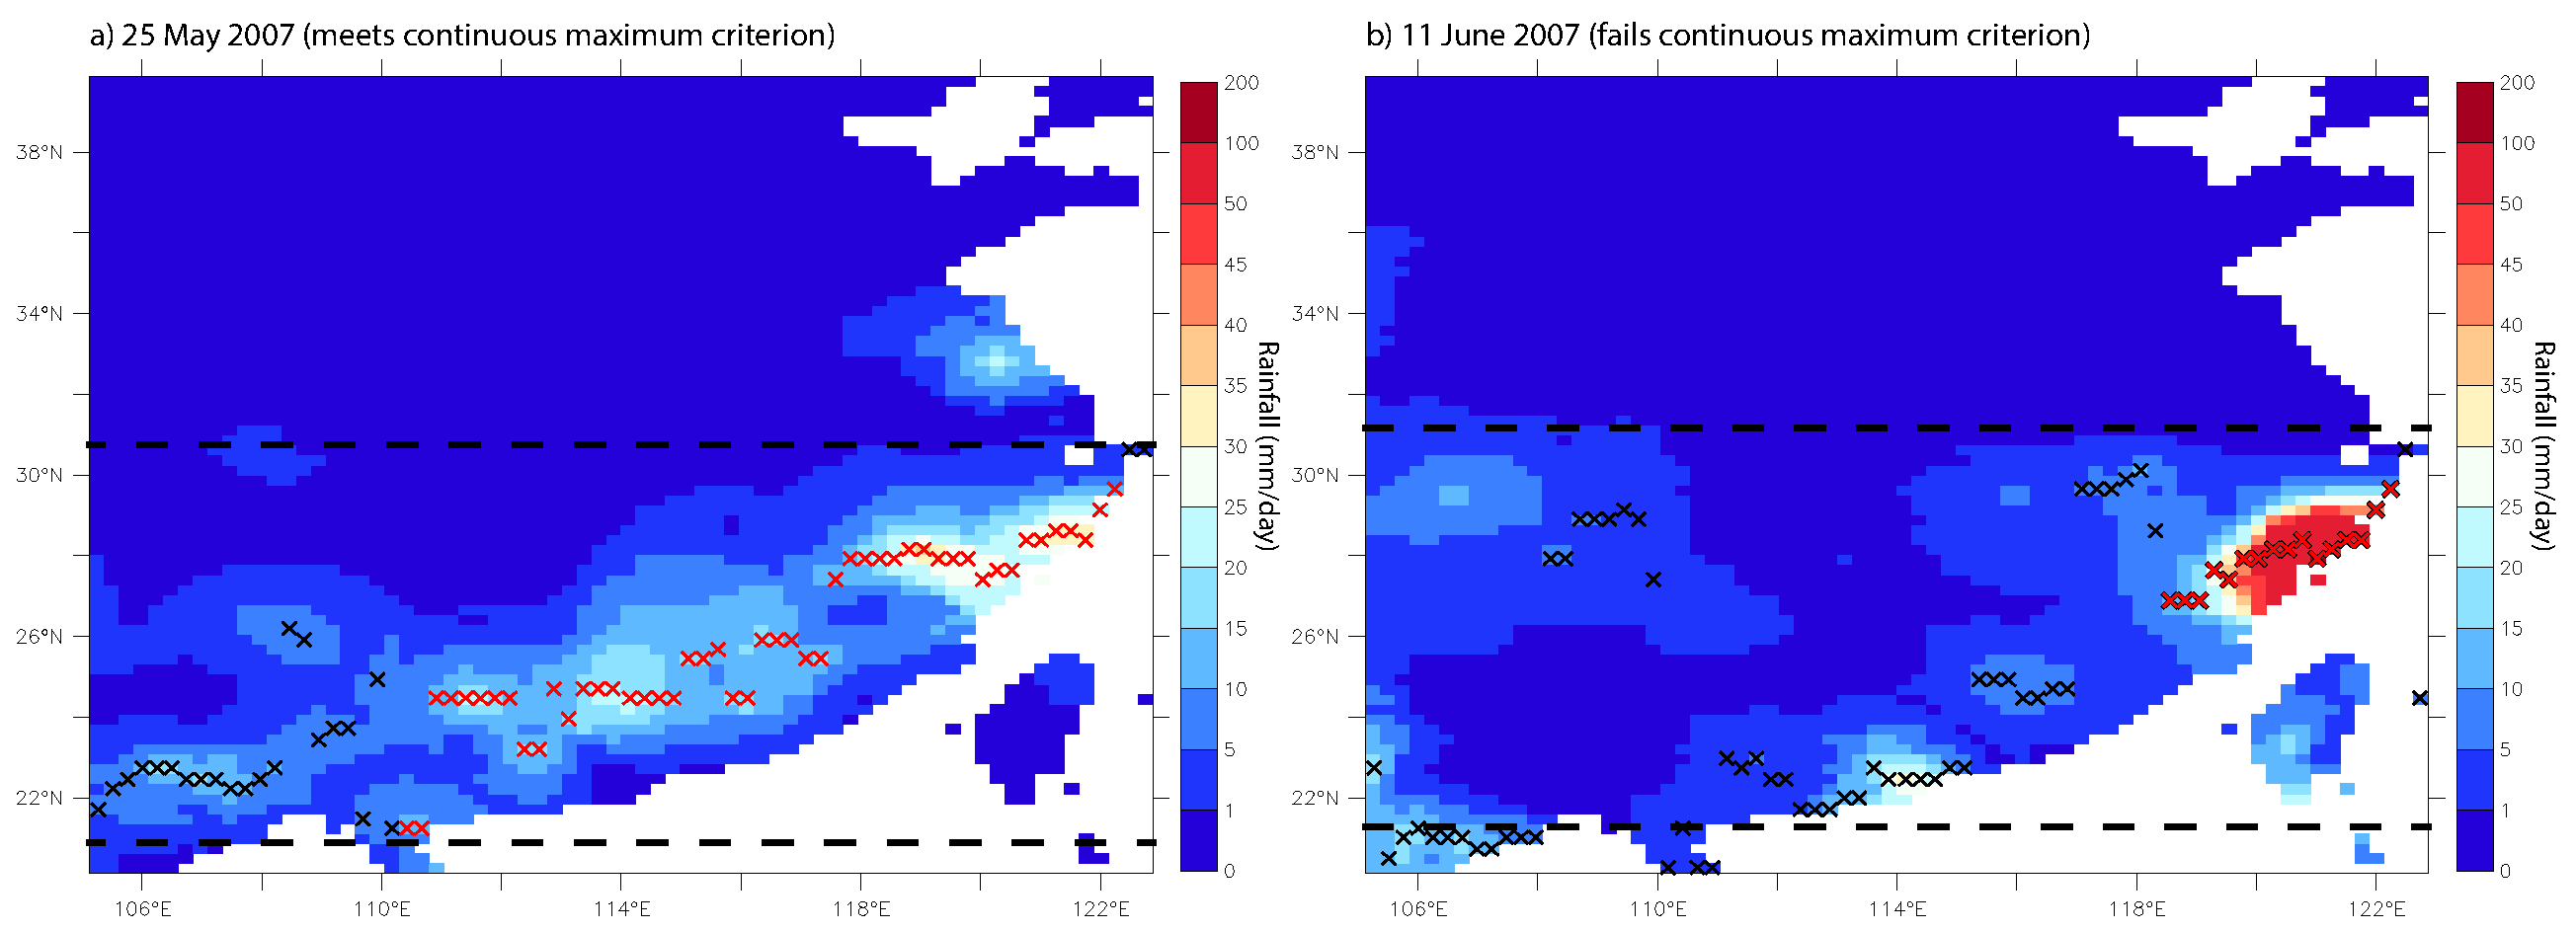
\includegraphics[width=36pc]{S1}
\caption{The first step of the rainband detection algorithm checks to see whether a five-degree continuous longitudinal band of precipitation maxima above 10 mm day$^{-1}$ exists. If so, a rainband fit is attempted. a) 25 May 2007 - the continuous maximum criterion is met and a fit is attempted. b) 11 June 2007 - although there is abundant rainfall in some locations, it appears not to be frontal and the continuous maximum criterion is failed. No fit is attempted.}
\end{figure}

%S2 - How the convergent fit algorithm works.
\begin{figure}
\setfigurenum{S2}  

\noindent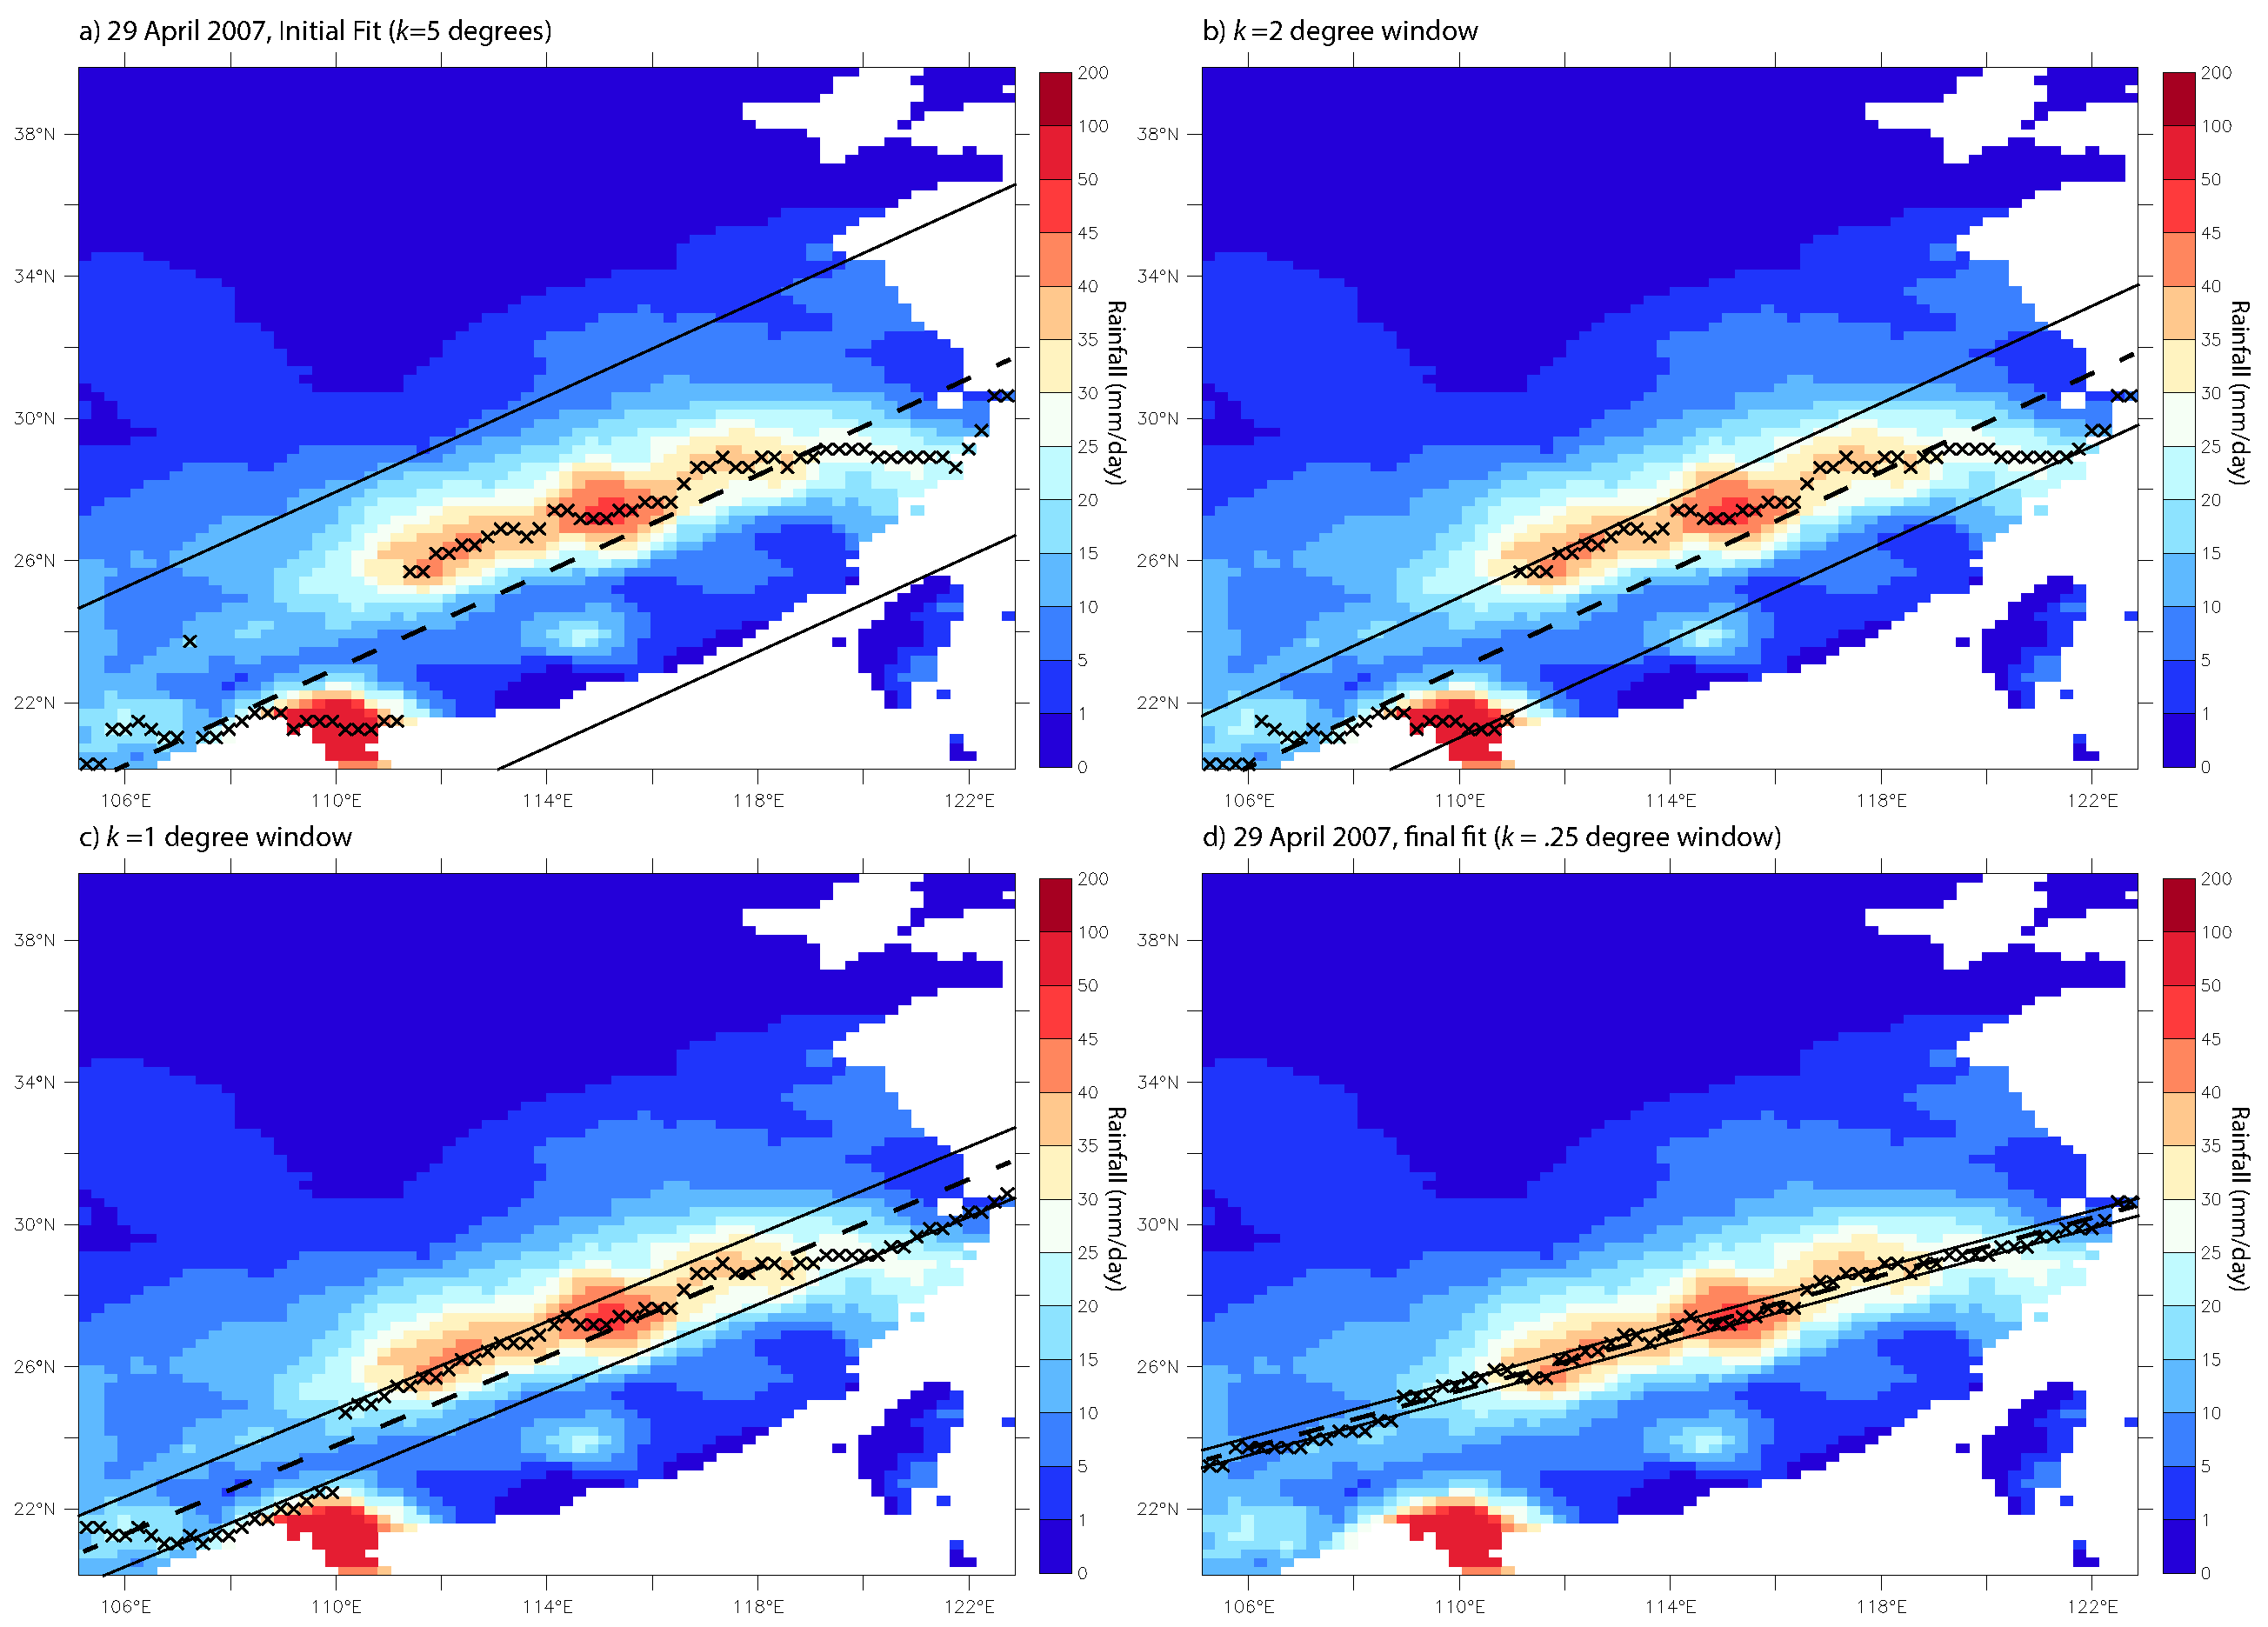
\includegraphics[width=36pc]{S2}
\caption{Display of the functionality of the recursive convergent algorithm. On 29 April 2007, a strong maximum in southernmost China skews our initial rainband fit (a), but the algorithm eventually converges on the most prominent coherent band via tighter windowing (d).}
\end{figure}

%S3 - Procedure for finding double rainbands
\begin{figure}
\setfigurenum{S3}  

\noindent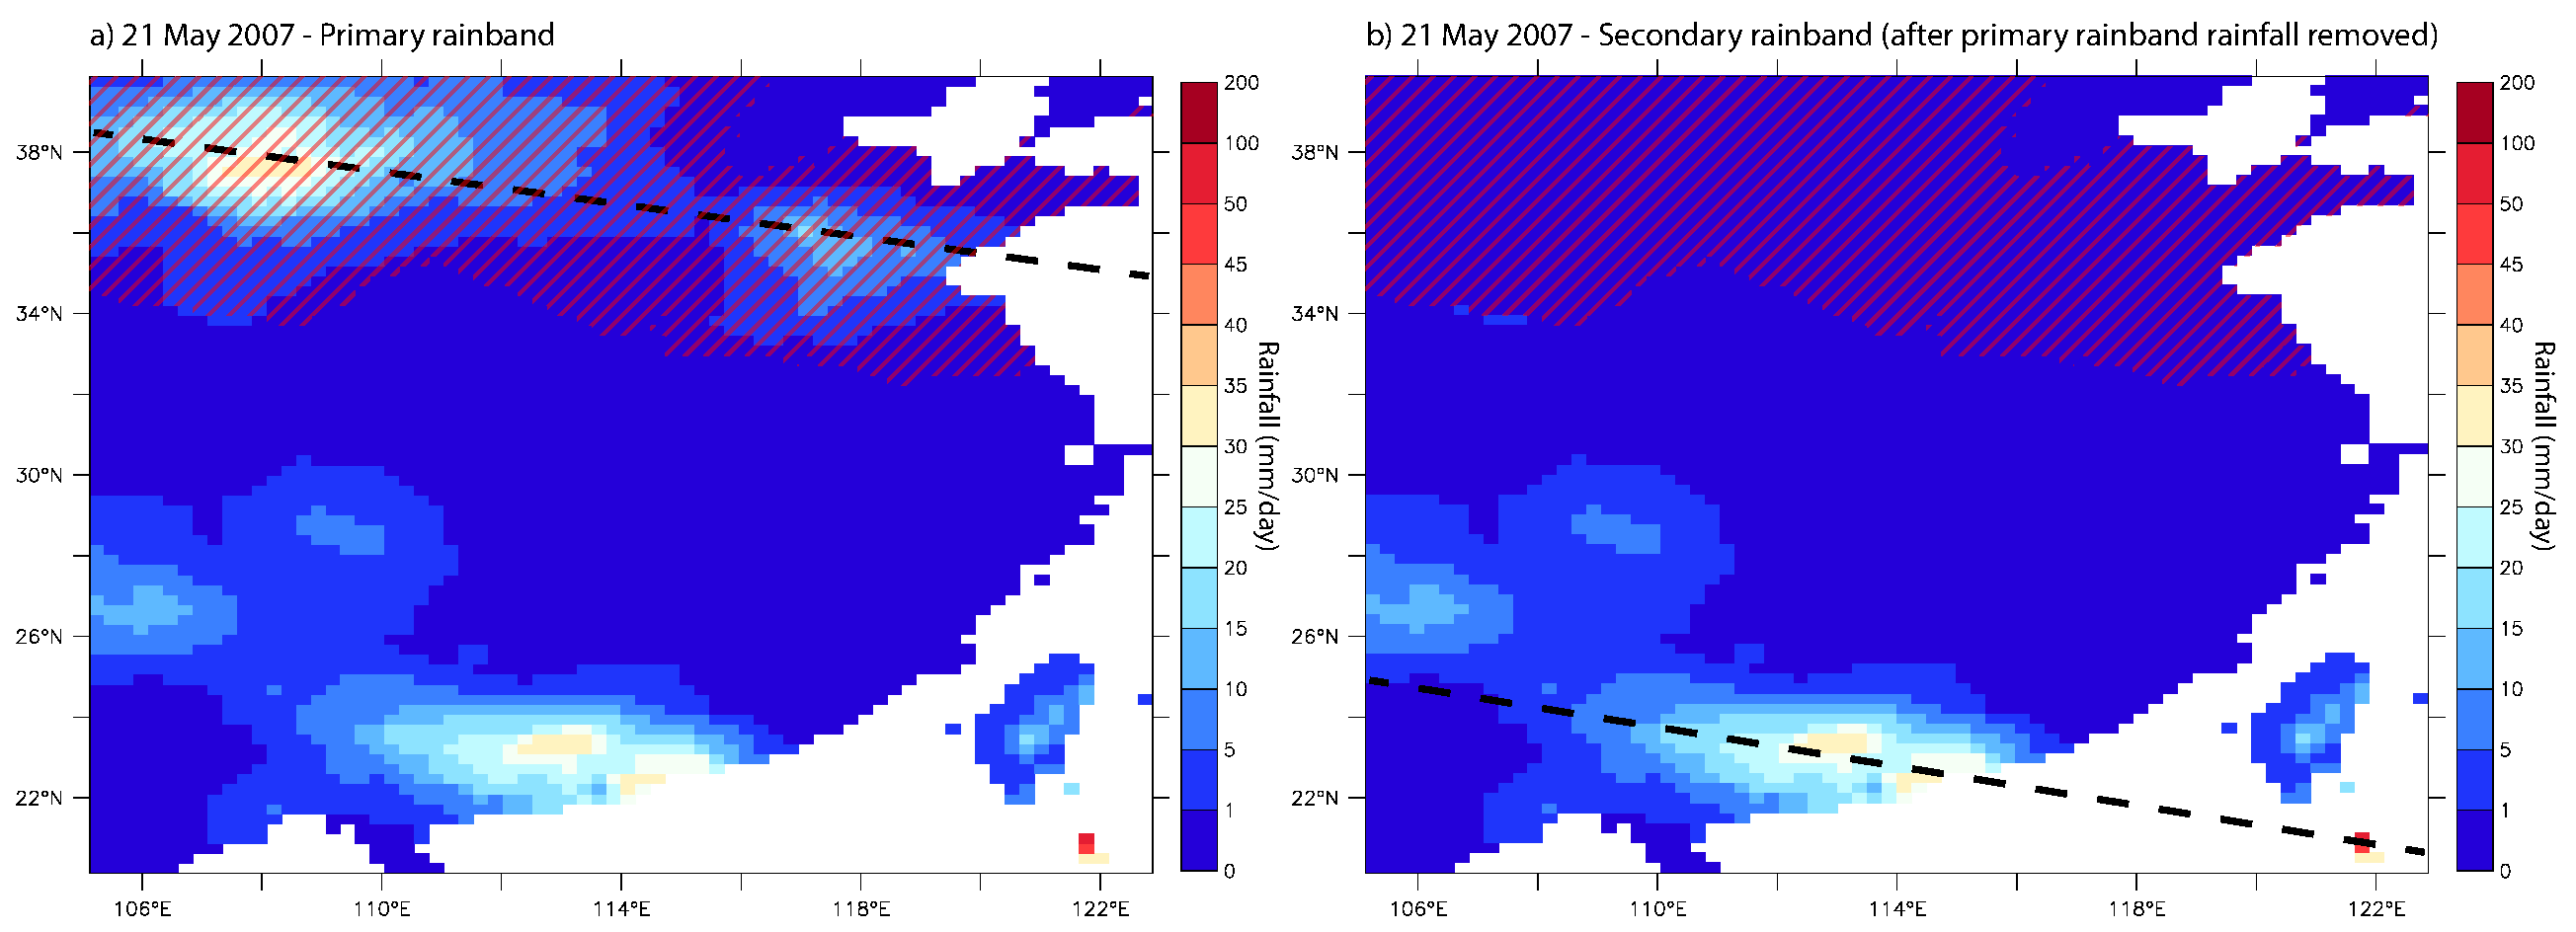
\includegraphics[width=36pc]{S3}
\caption{a) The algorithm converges on the strongest rainband, around 37N (defined as the ``primary rainband''). b) The rainfall associated with the primary rainband is removed, and we check for the presence of another rainband (a ``secondary rainband''), again using the continuous maximum criterion.}
\end{figure}

%S4 - Quality Control algorithm used to determine inclusion in statistics
\begin{figure}
\setfigurenum{S4}  

\noindent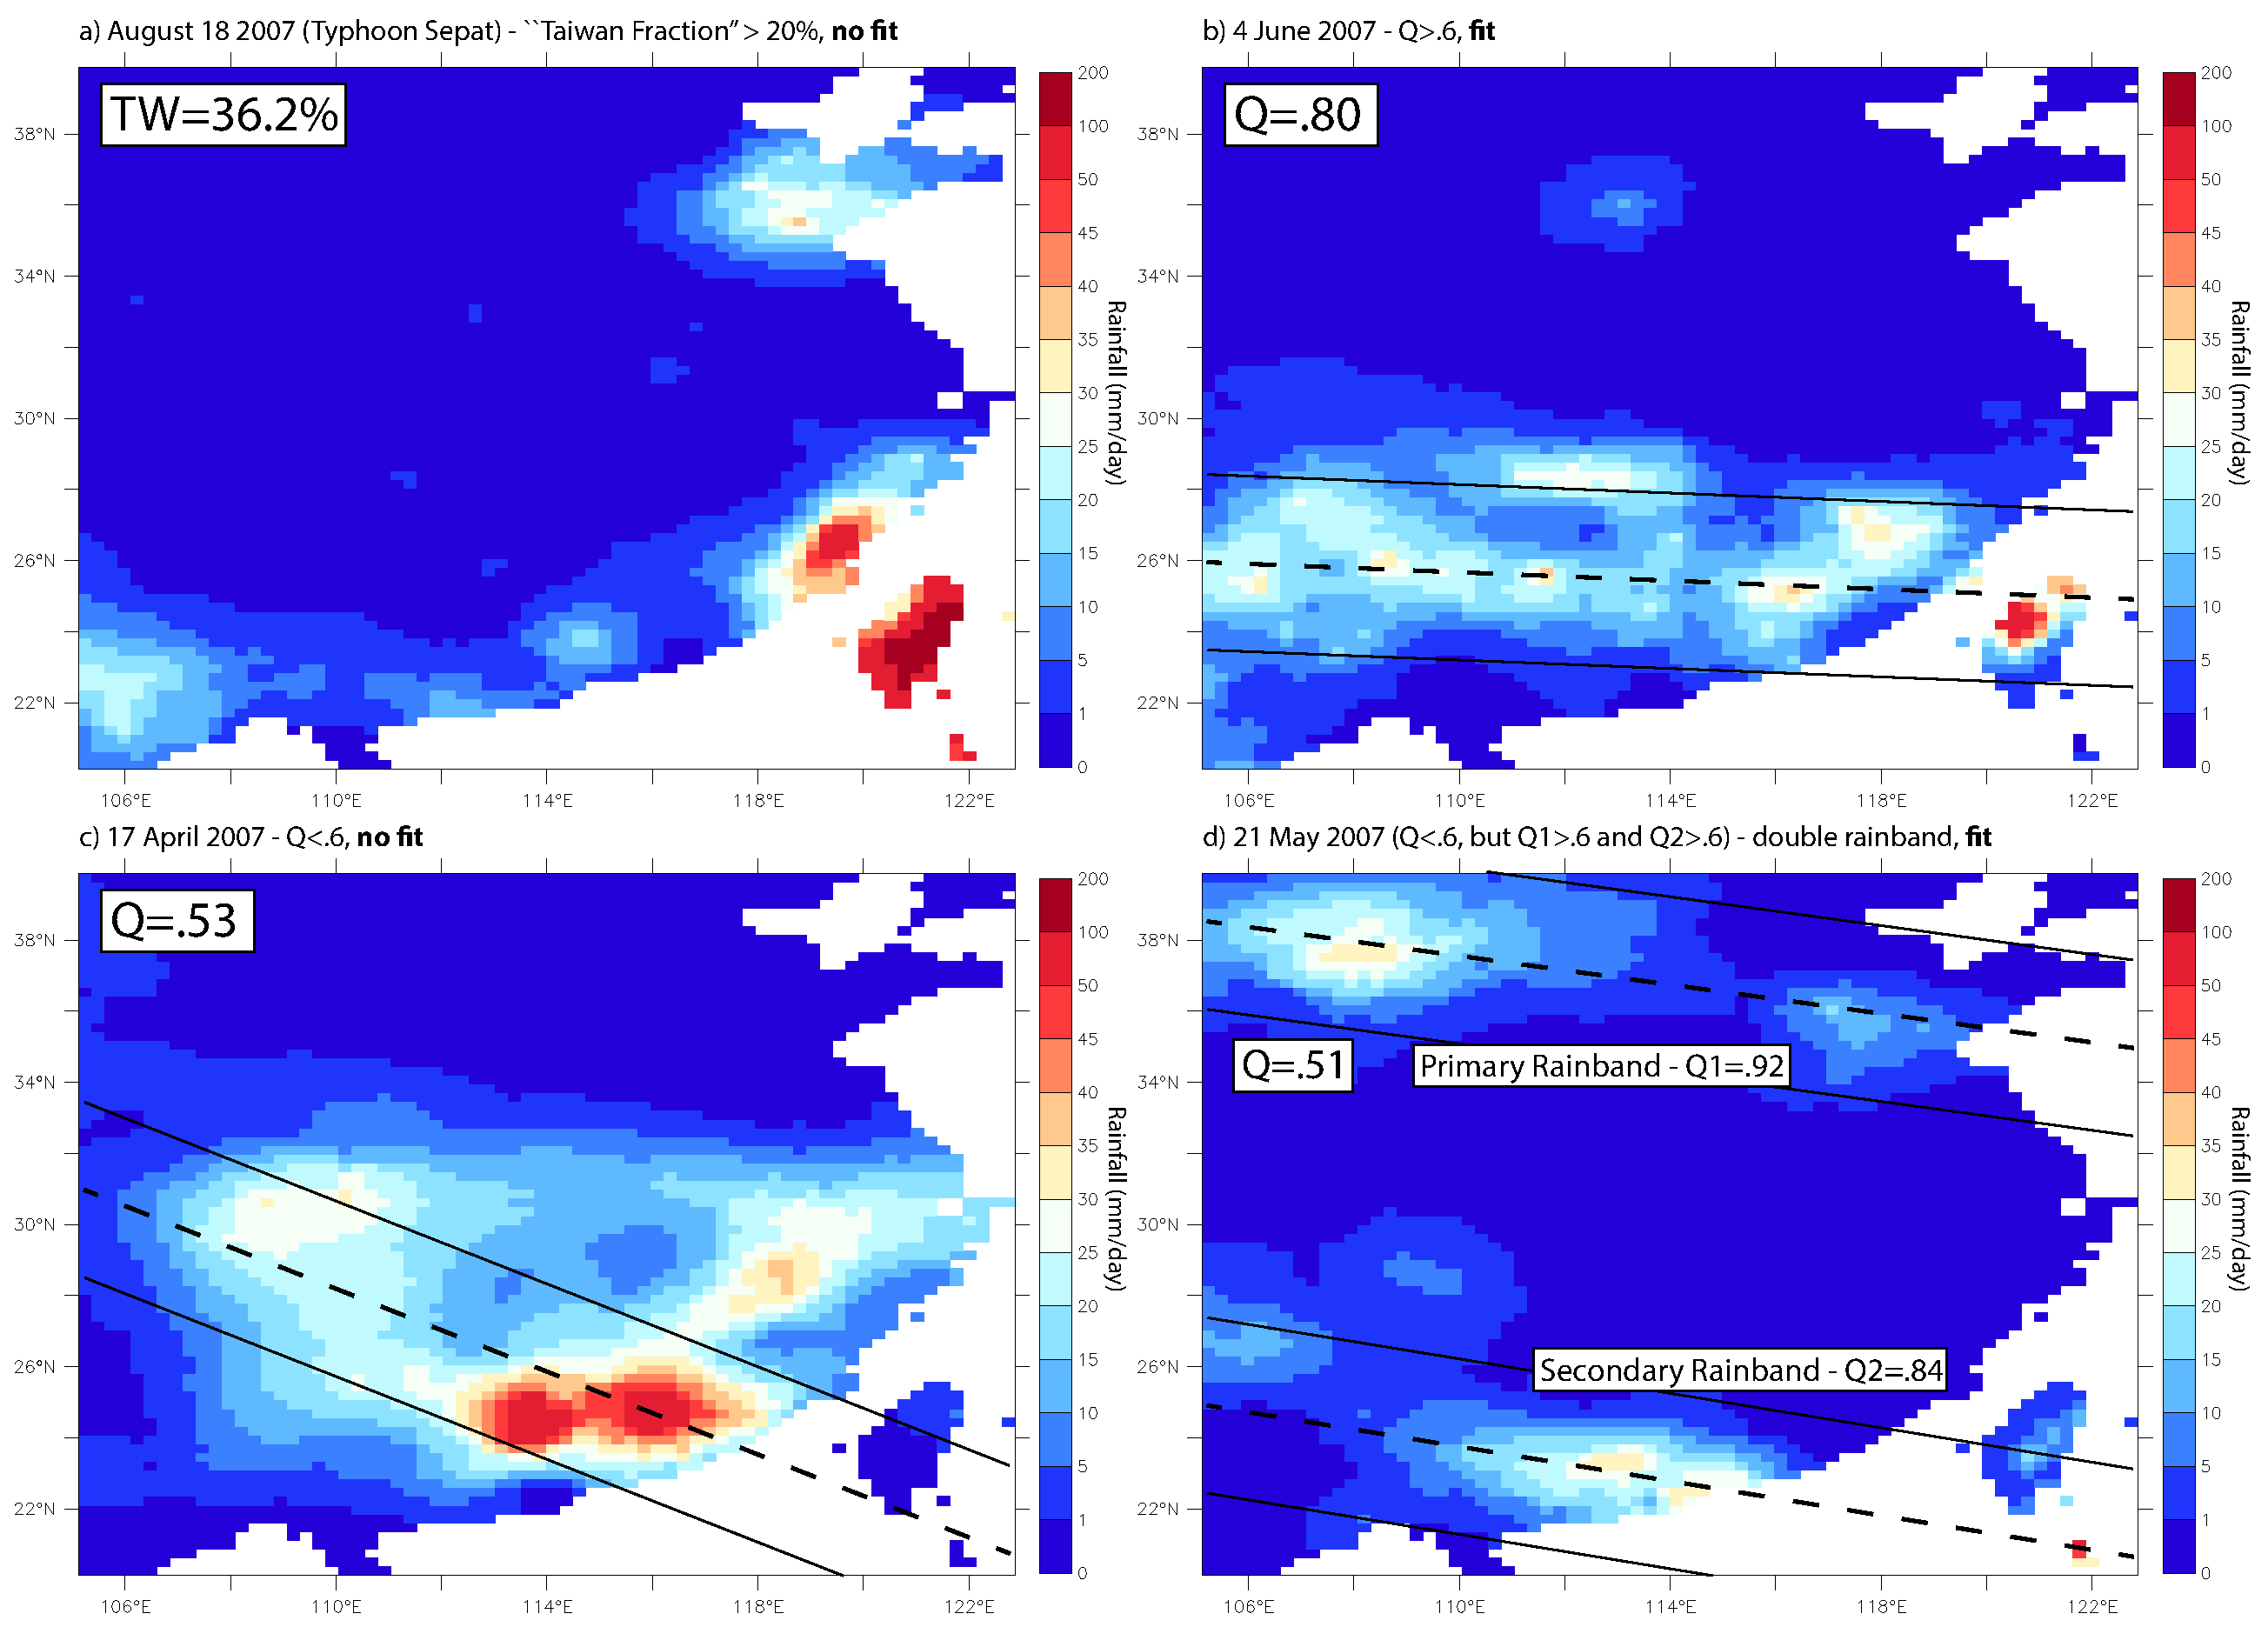
\includegraphics[width=36pc]{S4}
\caption{A quality control algorithm is used to exclude poor fits. a) 18 August 2007 - Days with a high Taiwan fraction (here, corresponding to the passage of Typhoon Sepat) are excluded from our statistics. b) June 4 2007 - A high-quality fit is achieved. c) 17 April 2007 - Although a fit is reached, it explains the distribution of daily rainfall poorly and is therefore excluded from rainband statistics. d) 21 May 2007 (same day as Figure S3) - An initial fit appears to be of poor quality ($Q<.6$). However, after finding a secondary rainband, we determine that conditional quality scores $Q_1$ and $Q_2$ are high, and the day is included in our statistics.}
\end{figure}


\end{document}
